\documentclass[usenames,dvipsnames,tikz]{standalone}
\usetikzlibrary{patterns}
%\usetikzlibrary{shapes.geometric}
%\usepackage{xcolor}
\colorlet{tBlue}{RoyalBlue!35!Cerulean}
\colorlet{tRed}{Red}
%\definecolor{tGreen}{HTML}{569909}
%\definecolor{tOrange}{HTML}{FA7602}
\usepackage{tikz}
\usepackage{standalone}
\begin{document}	
	
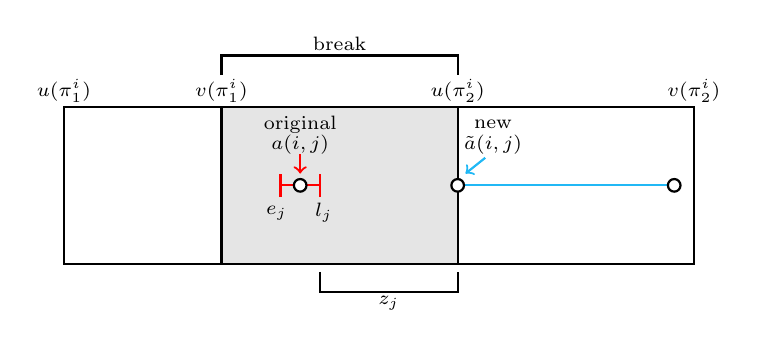
\begin{tikzpicture}
%\draw [help lines] (-1,-2) grid (15,7);

\draw [thick] (0,2) rectangle (8,4);
\draw [thick, fill=black!10!white] (2,2) rectangle (5,4);
%\draw [thick, pattern = north west lines, pattern color=black!40!white] (2,2) rectangle (5,4);
\draw [thick] (2,2) -- (2,4); % start of unavailable shift time
\draw [thick] (5,2) -- (5,4); % end of unavailable shift time

% Original job - duration 2.75, arrival 3 , start TW 2.75 , end TW 3.25 
\draw [thick, tRed] (2.75,3) -- (3.25,3); % line for TW of original job, length 0.5
\draw [thick, tRed] (2.75,2.85) -- (2.75,3.15); % vertical line for start of TW 
\draw [thick, tRed] (3.25,2.85) -- (3.25,3.15); % vertical line for end of TW
\draw [fill=white, thick] (3,3) circle [radius = 0.08]; % original arrival time at job
%\draw [fill=white, thick] (4,3) circle [radius = 0.08]; % original end time of job

% New job - duration 2.75, arrival/start 5, end 7.75
\draw [thick, tBlue] (5,3) -- (7.75,3); % line for duration of new job, length 2.75,
\draw [fill=white, thick] (5,3) circle [radius = 0.08]; % new arrival time at job
\draw [fill=white, thick] (7.75,3) circle [radius = 0.08]; % new end time of job

% Waiting time
%\draw [thick] (1.25, 1.9) -- (1.25, 1.65) -- (2, 1.65) -- (2,1.9);
%\node at (1.625, 1.5) {\scriptsize{waiting time}};

% Tardiness
\draw [thick] (3.25, 1.9) -- (3.25, 1.65) -- (5, 1.65) -- (5,1.9);
\node at (4.125, 1.5) {\scriptsize{$z_j$}};

% Unavailable time
\draw [thick] (2,4.4) -- (2,4.65) -- (5,4.65) -- (5,4.4);
\node at (3.5, 4.8) {\scriptsize{break}};

% Labels
\node at (0,4.2) {\scriptsize{$u(\pi_1^i)$}};
\node at (2,4.2) {\scriptsize{$v(\pi_1^i)$}};
\node at (5,4.2) {\scriptsize{$u(\pi_2^i)$}};
\node at (8,4.2) {\scriptsize{$v(\pi_2^i)$}};
\node at (3, 3.77) {\scriptsize{original}};
\node at (3, 3.52) {\scriptsize{$a(i,j)$}};
\draw [thick, tRed, ->] (3, 3.4) -- (3, 3.15);
\node at (2.7, 2.65) {\scriptsize{$e_j$}};
\node at (3.3, 2.65) {\scriptsize{$l_j$}};
\node at (5.45, 3.77) {\scriptsize{new}};
\node at (5.45, 3.52) {\scriptsize{$\tilde{a}(i,j)$}};
\draw [thick, tBlue, ->] (5.35, 3.35) -- (5.1, 3.15);







%\draw [thick] (0,0) rectangle (4,1.55);
%\draw [thick, dashed] (0.5,0) -- (0.5, 1.55);
%\draw [thick, dashed] (3,0) -- (3, 1.55);
%\node at (2,0.75) {\LARGE{$i$}};
%\draw [ultra thick, tBlue] (1,3) -- (1.8,3);
%\draw [tRed] (1.8,3) -- (2.8,3);
%\draw [fill=white, thick] (1,3) circle [radius = 0.08];
%\node [above] at (1,3.05) {\large{$v_1$}};
%\node at (1.025,2.5) {$4$};





\end{tikzpicture}
	
\end{document}


